%% Autor: Björn Ritterbecks 
%% Letzte Aenderung: 15.06.2016 
\thisfloatsetup{%
  capbesidewidth=\marginparwidth}
\begin{figure}[htbp]
\centering
%\sansmath
 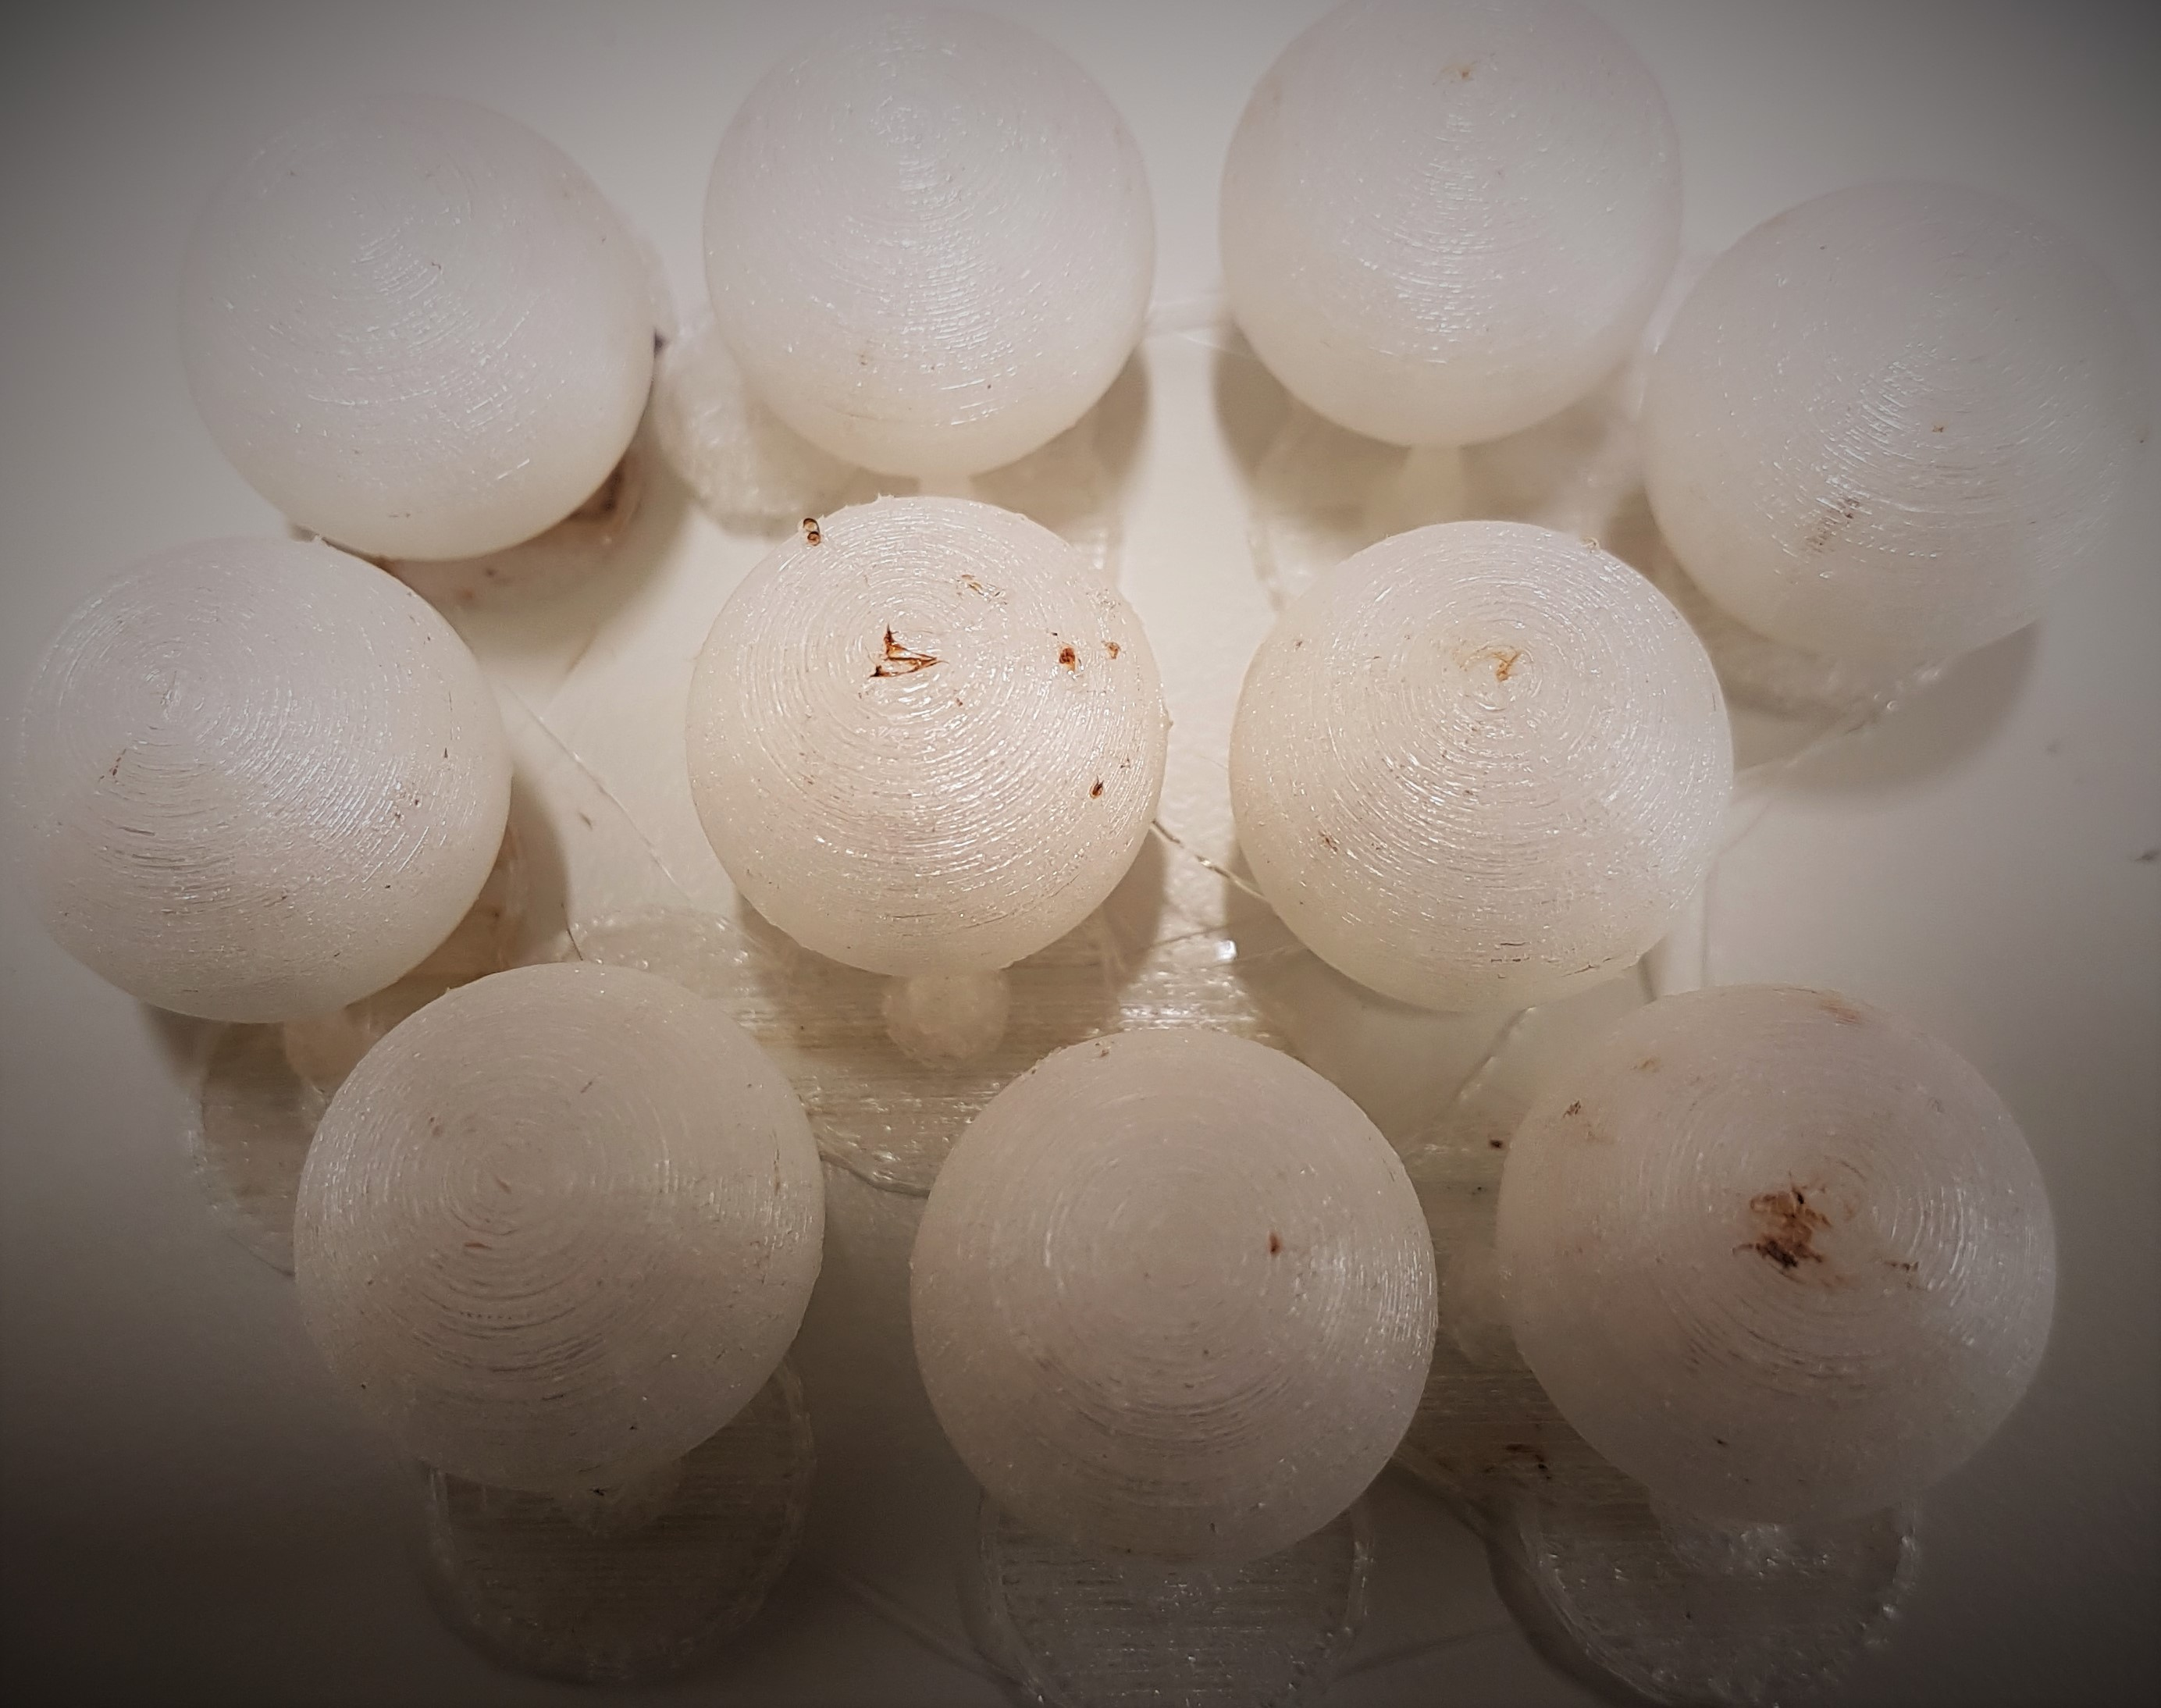
\includegraphics[width=0.99\textwidth]{images/gedrucktekugeln1.jpg}
  \caption[Probedruck der Kugeln]{Zu sehen ist ein Probedruck der Kugeln. Sie sind auf ein automatisiert berechnetes Stützensystem gedruckt, um den Druck der unteren Kugelhälften zu verbessern. Nicht zu sehen ist allerdings, dass die Unterseiten nicht symmetrisch, sondern abgeflacht sind.}
  \label{fig:gedrucktekugeln1}
  \vspace{-0pt}
\end{figure}